\documentclass[11pt]{article}
\usepackage[margin=1in]{geometry}
\usepackage{amsmath,amssymb}
\usepackage{booktabs,graphicx}
\usepackage[authoryear,round]{natbib}
\usepackage[colorlinks=true,allcolors=blue]{hyperref}

\title{Pre-FOMC Announcement Drift After 2020}
\author{}
\date{\today}

\begin{document}
\maketitle

\begin{abstract}
We test whether the pre-FOMC announcement drift survives after 2020 and whether it is concentrated in high-uncertainty meetings. Using S\&P~500 futures windows ending 15 minutes before the statement, a pre-specified state threshold (VIX 15.07, the development median) and a holdout of 52 scheduled meetings from 2020 to 2026 that was run once, we find a mean excess window return of 38.3~bps, far above matched-VIX non-meeting days (55.5~bps difference, $p=0.002$). The anxious-state premium of 37.8~bps is not distinguishable from zero with year-clustered wild-bootstrap inference ($p=0.149$), and the development finding that the premium is larger in anxious states does not replicate (contrast $-2.6$~bps, $p=0.946$), but the calm cell has only nine meetings and seven year clusters limit power. A verification of Federal Reserve release times also corrects the development benchmark: eight 2011--2012 meetings were released near 12:30 ET, and with the correct window the development mean falls from 6.2 to 2.8~bps and shows no post-2015 decline. The holdout result is unaffected.
\end{abstract}

\section{Introduction}
\citet{lucca2015} document large average excess equity returns in the 24 hours before scheduled FOMC policy statements, about 49~bps in 1994--2011, and subsequent work ties the premium to uncertainty \citep{hu2022,martello2018}. Three questions follow. Does the premium survive publication and the shift to press conferences at every meeting after 2019? Is it concentrated in high-uncertainty meetings, as the uncertainty-pricing account of \citet{hu2022} predicts? And are the original findings robust to how the announcement time is measured? A premium that shrinks after publication would be consistent with the decay of published predictors \citep{mclean2016}.

We fix the specification, state threshold and inference procedure in a pre-analysis plan, estimate on 2010--2019 intraday futures data, and run the 2020--2026 holdout once. In the holdout the mean excess window return is 38.3~bps and exceeds that on matched-VIX non-meeting days by 55.5~bps ($p=0.002$). The anxious-state premium is 37.8~bps but is not distinguishable from zero with year-clustered wild-bootstrap inference ($p=0.149$), and the anxious-minus-calm contrast is $-2.6$~bps ($p=0.946$), against $+19.2$~bps in development. With seven clusters and nine calm meetings the holdout has limited power, so we report bounds rather than evidence of absence.

A second contribution is measurement. Checking each development meeting against Federal Reserve release pages, we find that eight 2011--2012 meetings with press conferences released the statement at 12:20--12:35 ET rather than 14:15 ET, so the frozen window end followed the announcement for those meetings. We correct the development benchmark in a documented post-freeze amendment. The corrected development mean is 2.8~bps rather than 6.2, and the 2010--2014 versus 2015--2019 decline disappears. The holdout, whose statements are released at 14:00 ET, is unaffected. The paper is a disciplined out-of-sample check, not a causal estimate.
\section{Related literature}
\citet{lucca2015} report large average excess equity returns before scheduled FOMC announcements: about 49~bps over the 24 hours ending roughly 15 minutes before the announcement, across 131 scheduled meetings from September 1994 to March 2011 (as stated in the New York Fed staff report version). They find similar pre-announcement returns in other major equity indices but not in Treasuries or money market futures, and no comparable returns before other macroeconomic announcements. The effect is larger when the yield curve is flat, when the VIX is high and when past pre-FOMC returns were high.

\citet{hu2022} study overnight returns before nonfarm payrolls, ISM and GDP releases and propose that heightened uncertainty about the impact of upcoming news, proxied by the VIX, is priced and then resolves at the announcement. \citet{martello2018}, a 2018 master's dissertation at PUC-Rio (SSRN 3286745), studies state dependence of the FOMC premium on implied volatility: its introduction reports an average drift of 109~bps when implied volatility is above its prior median and 9.7~bps below, in a baseline sample of 60 scheduled meetings from September 2003 to March 2011. This is the closest antecedent to our state split, which is why we fix the threshold from the development sample rather than from the holdout.

A separate strand asks whether the drift reflects information leakage or monetary policy communication. \citet{cieslak2019} show that equity returns since 1994 concentrate in even weeks of the FOMC cycle and link this to informal communication between Fed officials and market participants. \citet{bernile2016} find abnormal E-mini S\&P~500 futures trading during FOMC news embargoes that predicts later policy surprises. \citet{kurov2019} find signs of informed trading before about nine of twenty market-moving announcements. If such channels operate, measured premia depend on communication and compliance regimes, which changed with the move to a press conference after every meeting from 2019 \citep{boguth2019}. That paper reports that announcements with a press conference move prices more and that the market risk premium is higher on press conference days, which matters here because every 2020--2026 meeting had one.

\citet{mclean2016} study 97 cross-sectional predictors and report portfolio returns 26\% lower out of sample and 58\% lower post-publication. They study cross-sectional predictors, not announcement-window returns, so we use them only as a benchmark for expected decay. Our holdout tests the state-dependent prediction on data that none of these papers used.
\section{Data}\label{sec:data}
\textbf{Prices.} The outcome is built from S\&P~500 e-mini futures last-trade prices on a fixed Eastern-time grid (09:45, 12:00, 13:30, 13:45, 14:00, 14:15, 14:30, 15:45, 16:00), obtained from Databento. SPY from WRDS TAQ cross-checks the grid on 2010--2017 development days (correlation 0.997 of 24-hour log returns, differences explained by ex-dividend days and one bad SPY print). Contract rolls are flagged and excluded. Futures trade nearly 24 hours, so the window return is measured from the 16:00 cash close of the previous valid session. The outcome is the log return from that print to the print at the window end on the meeting day, net of the daily risk-free rate, in basis points.

\textbf{Window end.} The window ends 15 minutes before the statement. From 2013-03-01 the statement is released at 14:00 ET and the end is 13:45; before that, statements were released at 14:15 and the end is 14:00. Per-meeting release times were checked against Federal Reserve pages for the meetings where the rule could fail: eight 2011--2012 press-conference meetings released the statement at 12:20--12:35 ET (listed in the replication data), and for these the window ends at 12:00. The holdout uses 13:45 throughout.

\textbf{State and samples.} The state variable is the VIX close five trading days before the meeting. The development sample covers 77 scheduled meetings from 2010-06 to 2019 and 2{,}239 non-meeting days; the holdout covers 2020--2026 with 53 scheduled meetings, of which 52 pass the validity filter. Unscheduled meetings are excluded. Half-day sessions, days with missing trades and futures roll windows are flagged and excluded by the panel builder, which logs row counts at every merge. The anxious threshold is the development-sample median VIX, 15.07; since it depends only on the VIX, it is unchanged by the release-time correction. Intraday data before 2010 are unavailable to us, so the original 1994--2011 evidence enters as published results, not as an estimate. A press conference was held at every 2019 and 2020 meeting, so the press-conference regime is constant in the holdout.
\section{Empirical Design}

\subsection{Identification}
The object of interest is the return earned in the window that ends before the
FOMC statement is released, in excess of the risk-free rate. Close-to-close daily
returns include the announcement reaction and therefore measure a different
quantity, so the primary test uses intraday prices. The comparison of interest is
between meetings held in calm and in anxious states, where the state is the VIX
close five trading days before the meeting (lagged one week) and the anxious
threshold is fixed at the development-sample median of 15.07 VIX points. The
threshold is not re-estimated on the holdout. The secondary specification
replaces the indicator with the continuous lagged VIX.

Identification rests on the timing of the window and on the state being
predetermined. Lagging the state by a week limits contamination from
anticipation of the meeting itself. The claim is a conditional association
between pre-announcement returns and the prior volatility state, not a causal
effect of the Committee's actions, and the paper is framed accordingly.

\subsection{Threats to inference}
\paragraph{Episode clustering.} Anxious meetings concentrate in a small number of
volatility episodes, so the effective number of independent observations is far
smaller than the number of meetings. We cluster by calendar year as an
ex-ante proxy for episodes, use CR1 cluster-robust standard errors, and treat
the wild cluster bootstrap-t as primary because the holdout has few clusters.
Asymptotic $t$ statistics are descriptive only.

\paragraph{Power.} With a small number of independent episodes the design can
detect a large premium but cannot distinguish a half-sized premium from zero. We
therefore report minimum detectable effects from a clustered power simulation
using realized volatility, and present non-rejections as bounds on the premium
rather than as evidence of absence.

\paragraph{Release-time measurement.} Statement release times are assigned by
rule rather than observed per meeting, so the window may include a few minutes of
the announcement reaction in some early meetings. This affects the level of the estimate more than the state comparison.
\emph{Update (verified against Federal Reserve release pages).} Eight development meetings
(2011-04-27, 2011-06-22, 2011-11-02, 2012-01-25, 2012-04-25, 2012-06-20, 2012-09-13,
2012-12-12) released the statement at about 12:20--12:35~ET, not 14:15~ET, so their 14:00 window
end follows the announcement. The holdout (2020 onward) is unaffected: its statements are
released at 14:00~ET. Appendix~\ref{app:sens} reports the development-sample effect of this error.

\paragraph{Non-FOMC confounds.} A premium measured on FOMC days could reflect
generic high-volatility or pre-event compensation. The matched-VIX placebo
compares FOMC windows with non-FOMC windows on days with similar lagged VIX, so a
Fed-specific premium requires an excess over matched days.

\paragraph{State measurement.} VIX comparability has changed over time as
short-dated option volume has grown. This matters mainly for the exploratory
VIX-change test, which is outside the frozen specification.

\paragraph{Specification search.} The specification, threshold, outcome window and
inference procedure are fixed in the pre-analysis plan before any estimate on
post-2019 data, and the holdout is run once. Tests outside the plan are labelled
exploratory and cannot change the primary conclusion.

\section{Results}
All holdout estimates come from a single run of the frozen specification; secondary tests are labelled exploratory. The development column uses the corrected release times (Section~\ref{sec:amend}). Standard errors are clustered by year (seven clusters), so we report wild cluster bootstrap $p$-values alongside.

\paragraph{Primary holdout test.} Table~\ref{tab:primary} reports the primary specification. The anxious-state premium is 37.8~bps ($t=1.91$, wild $p=0.149$) against 12.6~bps in development; its sign matches development but it does not reject zero at 5\%. The key contrast $b$ (anxious minus calm) is $-2.6$~bps (wild $p=0.946$): it does not replicate the development difference of 19.2~bps (wild $p=0.057$). The reason is the calm cell, whose mean rises from $-6.6$ to 40.4~bps. That cell has only nine meetings, so $b$ is weakly identified (Figures~\ref{fig:scatter} and~\ref{fig:state}). The continuous VIX slope is 5.02~bps per point ($t=2.48$) against 1.87 in development, but it is a single-sample, seven-cluster estimate and two high-VIX meetings in 2020 are visible leverage points in Figure~\ref{fig:scatter}. The matched-VIX placebo on non-meeting days gives a Fed-minus-matched difference of 55.5~bps ($p=0.002$) for all meetings and 38.3~bps ($p=0.030$) for anxious meetings, so the window return around meetings exceeds that on comparable non-meeting days. In development the same placebo shows no Fed-specific premium ($-11.9$~bps, $p=0.65$).

\begin{table}[ht]\centering\caption{Primary specification, development and holdout. Standard errors (year-clustered) in parentheses. Placebo sample sizes shown are for the holdout; development has 77, 38 and 39 meetings.}\label{tab:primary}
\small\begin{tabular}{lrr}\toprule
 & Development (corrected) & Holdout \\ \midrule
Calm mean $a$ (bps) & $-6.6$ (3.3) & 40.4 (5.4) \\
Anxious$-$calm $b$ (bps) & 19.2 (8.3) & $-$2.6 (21.9) \\
Anxious premium $a+b$ (bps) & 12.6 (7.5) & 37.8 (19.8) \\
Wild-bootstrap $p(b=0)$ & 0.057 & 0.946 \\
Wild-bootstrap $p(a+b=0)$ & --- & 0.149 \\
VIX slope $c$ (bps/pt) & 1.87 (1.05) & 5.02 (2.02) \\
\midrule
Placebo (all, $n=52$): Fed$-$matched (bps) & $-$11.9 ($p=0.65$) & 55.5 ($p=0.002$) \\
Placebo (anxious, $n=43$): Fed$-$matched (bps) & $-$12.0 ($p=0.81$) & 38.3 ($p=0.030$) \\
Placebo (calm, $n=9$): Fed$-$matched (bps) & $-$10.8 ($p=0.59$) & 35.2 ($p=0.209$) \\
\bottomrule\end{tabular}\end{table}

\begin{figure}[ht]\centering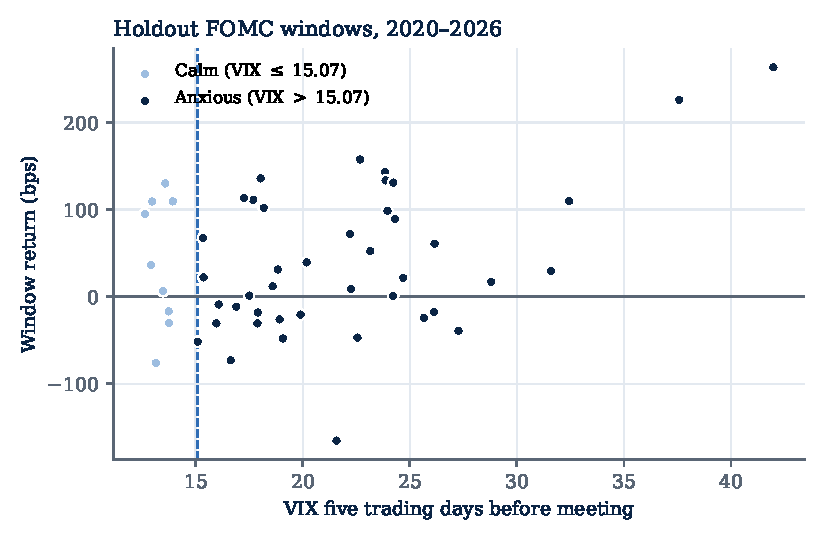
\includegraphics[width=.8\linewidth]{figures/fig1_holdout_scatter.pdf}\caption{Holdout meeting-window returns against lagged VIX.}\label{fig:scatter}\end{figure}
\begin{figure}[ht]\centering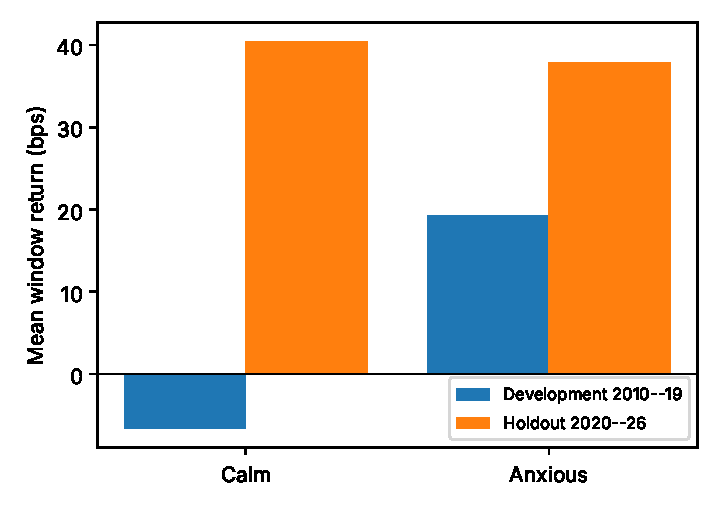
\includegraphics[width=.6\linewidth]{figures/fig2_state_means.pdf}\caption{Mean window return by state, development versus holdout.}\label{fig:state}\end{figure}

\paragraph{Exploratory secondary tests.} The VIX-change test finds no effect: the slope on the five-day VIX change is $-3.39$ ($t=-0.47$, wild $p=0.876$). The press-conference subsample (45 meetings from 2021 on) gives an anxious premium of 28.3~bps (wild $p=0.221$). The Federal Reserve held a press conference at every 2020 meeting too, which we verified only after the single run, so the subsample excludes 2020 for that reason; since the indicator equals one for all 52 holdout meetings, the subsample test adds nothing beyond the primary result and no comparison with non-press meetings is possible. Table~\ref{tab:robust} shows the anxious premium across thresholds, leave-one-year-out samples, winsorizing and no risk-free adjustment. It ranges from 26.6 to 69.5~bps. No wild $p$-value falls below 0.05, and the smallest is 0.092.

\begin{table}[ht]\centering\caption{Robustness of the holdout anxious premium (exploratory).}\label{tab:robust}
\small\begin{tabular}{lrrrrr}\toprule
Specification & $n$ & $n_{\mathrm{anx}}$ & Prem. (bps) & s.e. & Wild $p$ \\ \midrule
press=1 anxious premium & 45 & 37 & 28.3 & 20.5 & 0.221 \\
2021+ (flag-known sample) & 45 & 37 & 28.3 & 20.5 & 0.221 \\
baseline thr 15.07 & 52 & 43 & 37.8 & 19.8 & 0.149 \\
threshold 18 & 52 & 30 & 51.6 & 20.7 & 0.092 \\
threshold 20 & 52 & 23 & 59.2 & 22.3 & 0.194 \\
threshold 25 & 52 & 9 & 69.5 & 30.4 & 0.51 \\
holdout-median threshold & 52 & 26 & 48.7 & 25.2 & 0.284 \\
drop 2020 & 45 & 37 & 28.3 & 20.5 & 0.221 \\
drop 2021 & 44 & 35 & 51.9 & 17.2 & 0.114 \\
drop 2022 & 44 & 35 & 26.6 & 20.4 & 0.256 \\
drop 2023 & 44 & 39 & 41.6 & 21.7 & 0.199 \\
drop 2024 & 44 & 39 & 34.8 & 21.9 & 0.251 \\
drop 2025 & 44 & 35 & 37.7 & 24.7 & 0.3 \\
drop 2026 & 47 & 38 & 43.8 & 21.6 & 0.111 \\
excl 2020 (covid) & 45 & 37 & 28.3 & 20.5 & 0.221 \\
winsorized 5/95 & 52 & 43 & 35.9 & 16.2 & 0.121 \\
no rf adjustment & 52 & 43 & 38.8 & 19.8 & 0.135 \\
\bottomrule\end{tabular}\end{table}

\paragraph{Interpretation.} With seven clusters and nine calm meetings, the holdout is under-powered for the state contrast: the 80\% power minimum detectable effect for the anxious half is 40.3~bps at the corrected development volatility (21.8~bps for all holdout meetings). The evidence supports a positive meeting-window return, especially against matched non-meeting days. It does not confirm the development finding that the premium is concentrated in anxious states.


\subsection{Post-freeze amendment: development benchmark}\label{sec:amend}
After the holdout was run, a check of Federal Reserve release pages showed that eight 2011--2012 development meetings released the statement near 12:30 ET (Section~\ref{sec:data}), so the frozen window end of 14:00 ET followed the announcement. We therefore re-estimated the development benchmark only, with those eight windows ending at 12:00 ET; the frozen scripts, the threshold and the holdout are untouched. The development mean excess window return falls from 6.2 to 2.8~bps (clustered s.e.\ 4.6), the anxious premium from 19.3 to 12.6~bps, and the anxious-minus-calm contrast from 26.0 to 19.2~bps (wild $p=0.057$). The 2010--2014 and 2015--2019 means are now 2.9 and 2.8~bps, so the apparent post-2015 decline in the frozen run was produced by the eight mis-windowed meetings. The state contrast keeps its sign under every alternative window end (Appendix~\ref{app:sens}). Because the correction was made after seeing the holdout, we flag it as an amendment, not as part of the pre-registered plan; it changes what the holdout is compared with, not the holdout estimates.

\subsection{Exploratory: confidence intervals and pooled test}\label{sec:pooled}
These two analyses read the saved meeting-level files and were chosen after seeing the holdout, so they are exploratory. First, $t$-based 95\% confidence intervals with six degrees of freedom from the saved holdout estimates are $[27.2,\,53.6]$~bps for the calm mean, $[-10.6,\,86.2]$~bps for the anxious premium and $[-56.2,\,51.0]$~bps for the anxious-minus-calm contrast. The contrast interval is wide enough to contain both zero and the corrected development value of 19.2~bps, which is the sense in which the holdout is uninformative about state dependence. Second, pooling the 77 corrected development and 52 holdout meetings (17 year clusters) with a period fixed effect gives an anxious-minus-calm contrast of 13.2~bps (s.e.\ 8.8, wild $p=0.163$) and a VIX slope of 3.47~bps per point (s.e.\ 1.36, wild $p=0.075$), with the holdout level 31.0~bps above development. Pooling increases power but the state contrast is still not significant at 5\%, and the slope is borderline. We read this as suggestive, not confirmatory, evidence that returns rise with uncertainty.

\section{Discussion}
The holdout supports a positive meeting-window return, particularly relative to matched non-meeting days, but does not replicate the development finding that the premium is concentrated in anxious states. Three readings are consistent with the data. First, the premium may be roughly state-independent after 2020; the calm cell mean rose from $-6.6$ to 40.4~bps and the overall mean from 2.8 to 38.3~bps. Second, the state contrast may be present but undetectable: the calm cell has nine meetings and the minimum detectable effect for the anxious half is 40.3~bps. Third, the 2020--2022 episode, in which VIX was high and the communication regime changed, may dominate a seven-cluster sample. The data cannot separate these.

Limitations are as stated in the design: release times are assigned by rule, and for eight 2011--2012 development meetings the rule is wrong (the statement came at about 12:30~ET), which we corrected after the holdout run (Section~\ref{sec:amend}), clustering by year is a proxy for volatility episodes, and the VIX-change and press-conference tests are exploratory. The comparison with the post-publication decline in \citet{mclean2016} is loose: the holdout premium does not fall, but an announcement-window return is not a cross-sectional anomaly portfolio, and the sample is too small to measure a decline precisely.

\section{Conclusion}
A single pre-specified holdout run finds a positive pre-announcement return in 2020--2026 that exceeds matched non-meeting days, but it does not confirm that the premium is concentrated in high-uncertainty meetings. Power is limited by few independent episodes and a thin calm cell. Longer samples or per-meeting release times are the natural next steps.


\bibliographystyle{plainnat}
\bibliography{references}

\appendix
\section{Notation and Additional Material}
\label{app:notation}

\subsection{Notation}
All returns are in basis points unless stated. Meeting $m$ indexes scheduled FOMC meetings; $t(m)$ is the meeting date and $t(m)^{-}$ the previous valid session.

\begin{table}[ht]
\centering
\small
\begin{tabular}{@{}lp{0.58\textwidth}l@{}}
\hline
Symbol & Definition & Unit \\
\hline
$P_{\mathrm{prev}}$ & 16:00 ET last price on the previous valid session & index points \\
$P_{\mathrm{end}}$ & Last price at the end of the pre-announcement window: 13:45 ET (14:00 ET release, from 2013-03-01 and throughout the holdout) or 14:00 ET (14:15 ET release, earlier) & index points \\
$rf_m$ & Risk-free rate over the same interval (daily file) & bps \\
$r_m$ & Outcome: $10^{4}\,[\ln(P_{\mathrm{end}}/P_{\mathrm{prev}})] - rf_m$ & bps \\
$\mathrm{VIX}_m$ & VIX close five trading days before the meeting date & VIX points \\
$\tau$ & Anxiety threshold, fixed at 15.07 (development-sample median) & VIX points \\
$A_m$ & $\mathbf{1}\{\mathrm{VIX}_m > \tau\}$, the anxious indicator & 0/1 \\
$a$ & Intercept: premium in calm meetings & bps \\
$b$ & Anxious minus calm difference & bps \\
$a+b$ & Premium in anxious meetings (primary test statistic) & bps \\
$c$ & Slope of $r_m$ on $\mathrm{VIX}_m$ in the secondary specification & bps per point \\
$\varepsilon_m$ & Disturbance & bps \\
$g(m)$ & Cluster (calendar year, a provisional proxy for volatility episodes) & --- \\
$G$ & Number of clusters (about seven in the holdout) & --- \\
\hline
\end{tabular}
\caption{Variables and parameters.}
\end{table}

\subsection{Specifications}
Primary:
\begin{equation}
r_m = a + b\,A_m + \varepsilon_m, \qquad H_1: a+b>0 .
\end{equation}
Secondary, reported alongside and not substituted:
\begin{equation}
r_m = a + c\,\mathrm{VIX}_m + \varepsilon_m .
\end{equation}
Inference uses CR1 cluster-robust standard errors by $g(m)$, wild cluster bootstrap-$t$ (999 draws, seed 1) for $b=0$ and $a+b=0$, and a matched-VIX permutation placebo against non-FOMC days (2000 draws, seed 2). With few clusters the bootstrap $p$-values are primary and asymptotic $t$ statistics descriptive.

\subsection{Hypotheses}
\begin{description}
\item[H1] $a+b>0$ in the holdout.
\item[H2] The holdout anxious premium is below the development estimate of 19.3 bps.
\item[H3] $b>0$.
\end{description}

\subsection{Sample definitions}
Development sample: scheduled meetings from 2010-06 to 2019-12-31. Holdout: scheduled meetings from 2020-01-01. Unscheduled meetings are excluded. A meeting is usable if the meeting day and previous session are valid (no half-day, missing-trade or cash-closed flag) and $r_m$ and $\mathrm{VIX}_m$ are non-missing. Release times are a calendar rule, not observed per meeting (UNVERIFIED).

\end{document}
